\begin{frame}[allowframebreaks]{Principal Component Analysis (PCA)}
    \begin{itemize}
        \item Principal Component Analysis (PCA) is a method for optimally summarizing large, multi-dimensional datasets.
        \item PCA identifies a smaller number of dimensions (ideally 2) that retain most of the useful information present in the original data.
        \item The technique constructs a set of new variables, called Principal Components (PCs), which are linear combinations of the original variables.
        \item Each Principal Component represents a specific weighted sum of the original features. For example:
        \begin{equation*}
            \text{PC} = (10 \times \text{GeneA}) + (3 \times \text{GeneB}) + (-4 \times \text{GeneC}) + (-20 \times \text{GeneD}) + \ldots
        \end{equation*}
        \item By projecting the data onto these principal components, PCA reduces dimensionality while preserving as much variance (information) as possible.
    \end{itemize}

    \framebreak

    \begin{itemize}
        \item Principal Component Analysis (PCA) is a method for optimally summarizing large, multi-dimensional datasets.
        \item PCA identifies a smaller number of dimensions (ideally 2) that retain most of the useful information present in the original data.
        \item The technique constructs a set of new variables, called Principal Components (PCs), which are linear combinations of the original variables.
        \item Each Principal Component represents a specific weighted sum of the original features. For example:
        \begin{equation*}
            \textcolor{gray}{\text{PC}} = \textcolor{gray}{(}10 \textcolor{gray}{\times \text{GeneA}) + (}3 \textcolor{gray}{\times \text{GeneB}) + (}-4 \textcolor{gray}{\times \text{GeneC}) + (}-20 \textcolor{gray}{\times \text{GeneD}) + \ldots}
        \end{equation*}
        \item By projecting the data onto these principal components, PCA reduces dimensionality while preserving as much variance (information) as possible.
    \end{itemize}

    Simple example using 2 genes and 10 cells

\end{frame}

\begin{frame}[allowframebreaks]{How does PCA work?}    
    Simple example using 2 genes and 10 cells
    \vspace{1cm}
    \begin{columns}
    \begin{column}{0.5\textwidth}
        \begin{figure}
            \centering
            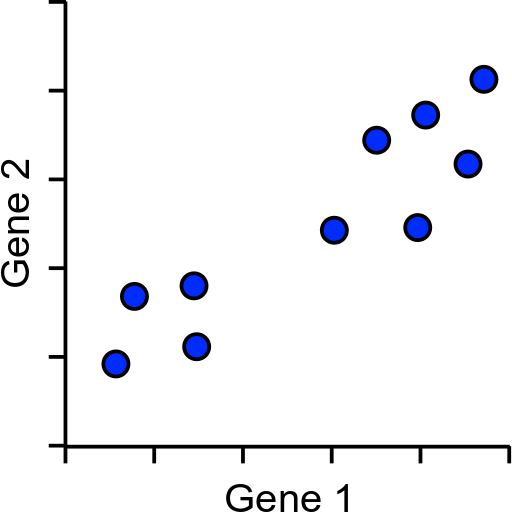
\includegraphics[width=1\textwidth,keepaspectratio]{images/dul/dim-reduce/points.png}
        \end{figure}
    \end{column}
    \begin{column}{0.5\textwidth}
        \begin{figure}
            \centering
            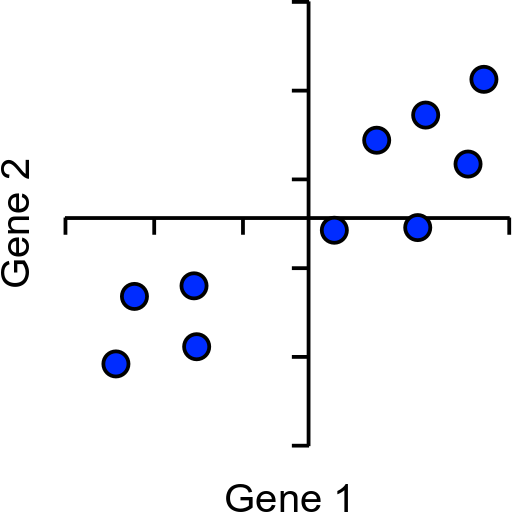
\includegraphics[width=1\textwidth,keepaspectratio]{images/dul/dim-reduce/points-separation.png}
        \end{figure}
    \end{column}
    \end{columns}

    \framebreak

    Find line of best fit, passing through the origin
    \vspace{1cm}
    \begin{columns}
    \begin{column}{0.33\textwidth}
        \begin{figure}
            \centering
            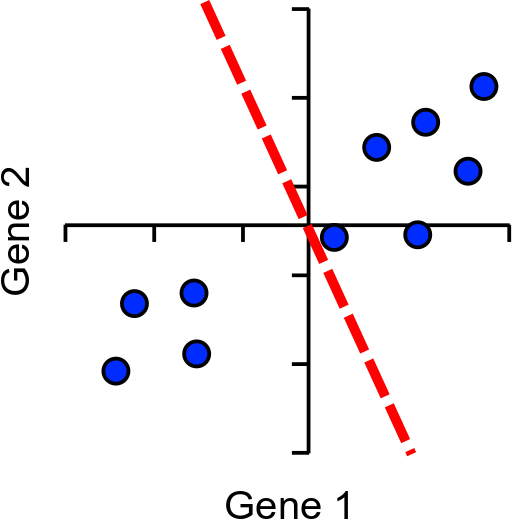
\includegraphics[width=1\textwidth,keepaspectratio]{images/dul/dim-reduce/line-fit.png}
        \end{figure}
    \end{column}
    \begin{column}{0.33\textwidth}
        \begin{figure}
            \centering
            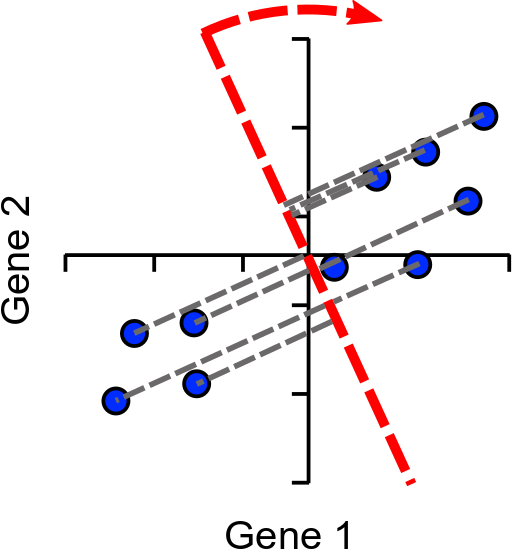
\includegraphics[width=1\textwidth,keepaspectratio]{images/dul/dim-reduce/line-fit-rotate.png}
        \end{figure}
    \end{column}
    \begin{column}{0.33\textwidth}
        \begin{figure}
            \centering
            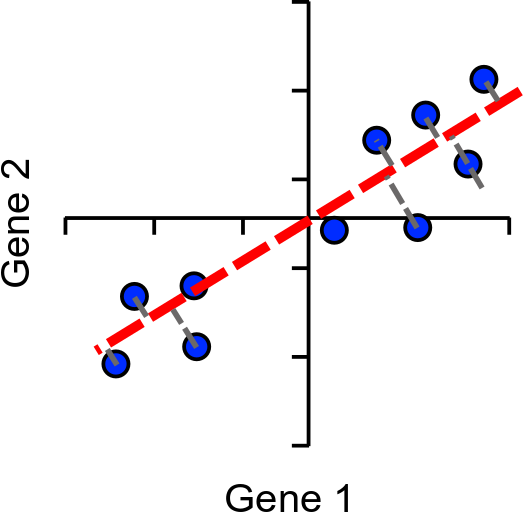
\includegraphics[width=1\textwidth,keepaspectratio]{images/dul/dim-reduce/line-fit-best.png}
        \end{figure}
    \end{column}
    \end{columns}
\end{frame}

\begin{frame}[allowframebreaks]{Assigning Loadings to Genes}    
    \begin{columns}
    \begin{column}{0.5\textwidth}
        \begin{figure}
            \centering
            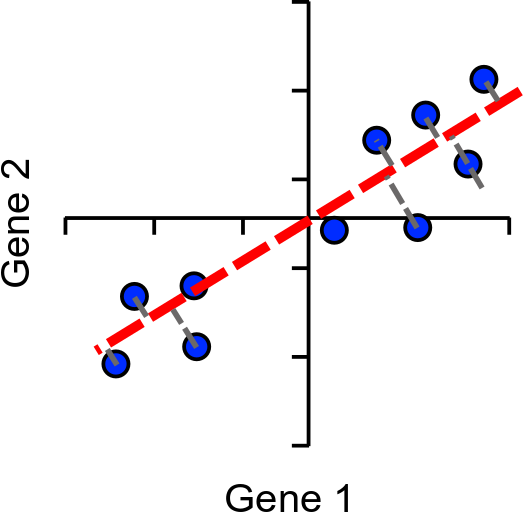
\includegraphics[width=0.8\textwidth,keepaspectratio]{images/dul/dim-reduce/line-fit-best.png}
        \end{figure}
    \end{column}
    \begin{column}{0.5\textwidth}
        \begin{figure}
            \centering
            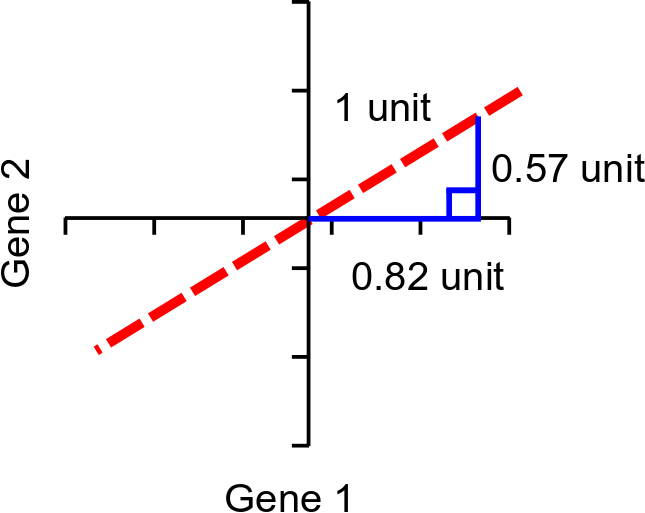
\includegraphics[width=0.8\textwidth,keepaspectratio]{images/dul/dim-reduce/line-eigenvector.png}
            \caption{\textbf{Eigenvector} or Single Vector}
        \end{figure}
    \end{column}
    \end{columns}
    \begin{itemize}
        \setlength{\itemsep}{-0.5em}
        \item \textbf{Loadings} represent the contribution of each gene to the principal component.
        \item For this example using 2 genes and 10 cells:
        \begin{itemize}
            \setlength{\itemsep}{-0.5em}
            \item Gene1 loading: $0.82$
            \item Gene2 loading: $0.57$
        \end{itemize}
        \item A higher loading means the gene has a greater influence on the principal component.
    \end{itemize}
\end{frame}


\begin{frame}[allowframebreaks]{More Dimensions}    
    \begin{columns}
    \begin{column}{0.4\textwidth}
        \begin{figure}
            \centering
            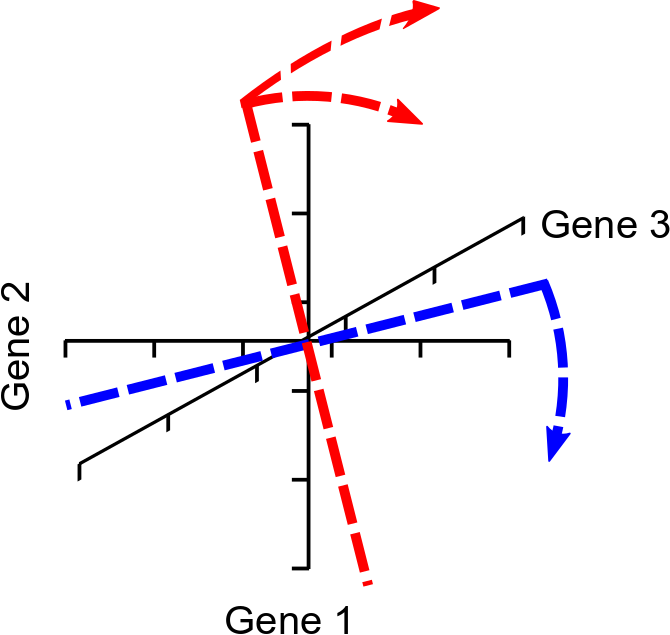
\includegraphics[width=1\textwidth,keepaspectratio]{images/dul/dim-reduce/multi-pcs.png}
        \end{figure}
    \end{column}
    \begin{column}{0.6\textwidth}
        \begin{itemize}
            \item The same idea extends to datasets with more dimensions ($n$ genes).
            \item The first principal component (PC1) finds the direction of maximum variance, rotating in $(n-1)$ dimensions.
            \item The next principal component (PC2) is perpendicular to PC1 and rotates in the remaining $(n-2)$ dimensions.
            \item Each subsequent principal component is always perpendicular to the previous ones, capturing the next largest variance.
            \item The last principal component is the only remaining perpendicular direction.
            \item The number of principal components always equals the number of original genes (features).
        \end{itemize}
    \end{column}
    \end{columns}
\end{frame}


\begin{frame}[allowframebreaks]{Explaining Variance}    
    \begin{itemize}
        \item Each principal component (PC) explains a certain proportion of the total variance in the data. Together, all PCs account for 100\% of the variance.
        \item PC1 always explains the largest amount of variance.
        \item PC2 explains the next largest amount, and so on for subsequent PCs.
        \item Since we typically plot only 2 dimensions (PC1 and PC2), it's important to check how much of the total variance these two PCs explain.
        \item \textbf{How do we calculate this?}
        % \begin{itemize}
        %     \item For each PC, divide the variance explained by that PC by the total variance (sum of variances of all PCs).
        %     \item This gives the proportion (or percentage) of variance explained by each PC.
        %     \item Often visualized using a \textit{scree plot} or by reporting the cumulative variance explained.
        % \end{itemize}
    \end{itemize}

    \framebreak

    \begin{columns}
    \begin{column}{0.5\textwidth}
        \begin{figure}
            \centering
            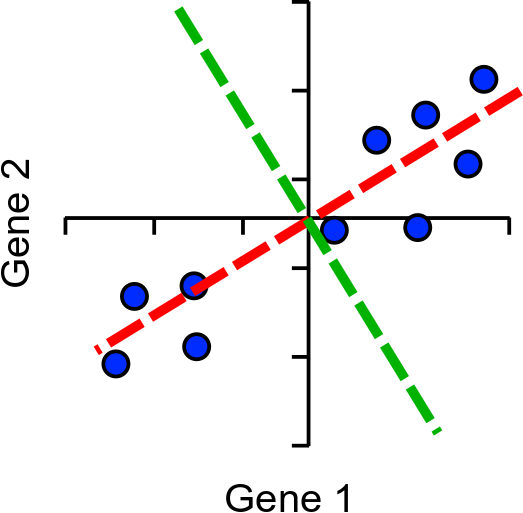
\includegraphics[width=1\textwidth,keepaspectratio]{images/dul/dim-reduce/variance-explained.png}
        \end{figure}
    \end{column}
    \begin{column}{0.5\textwidth}
        \begin{itemize}
            \item Project each data point onto the principal component (PC).
            \item Calculate the distance of each projected point to the origin.
            \item Compute the sum of squared differences (SSD) from the origin.
            \item This SSD is a measure of variance, called the \textit{eigenvalue}.
            \item Divide the SSD by $(\text{number of points} - 1)$ to obtain the actual variance explained by the PC.
        \end{itemize}
    \end{column}
    \end{columns}

    \framebreak

    \begin{columns}
    \begin{column}{0.5\textwidth}
        \begin{figure}
            \centering
            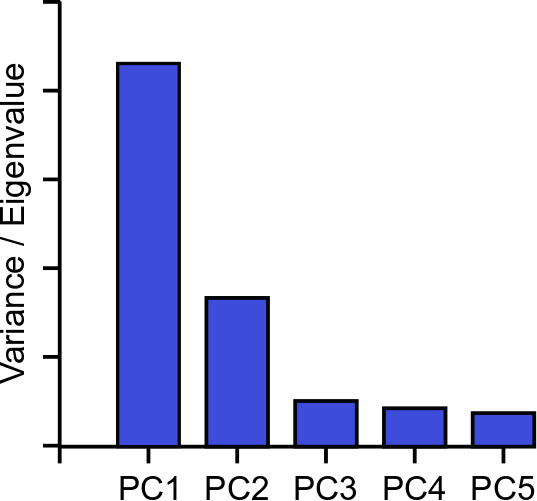
\includegraphics[width=1\textwidth,keepaspectratio]{images/dul/dim-reduce/variance-graph-1.png}
        \end{figure}
    \end{column}
    \begin{column}{0.5\textwidth}
        \begin{figure}
            \centering
            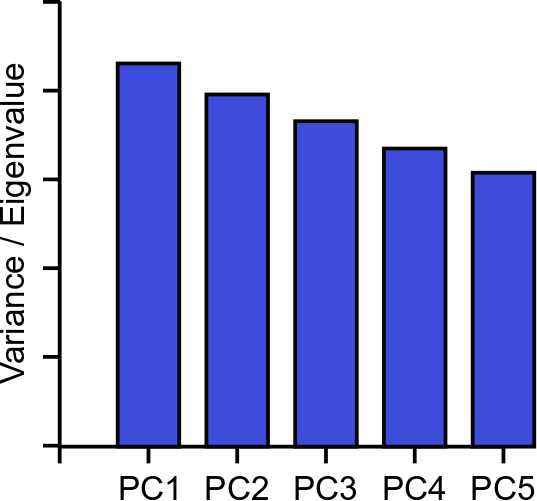
\includegraphics[width=1\textwidth,keepaspectratio]{images/dul/dim-reduce/variance-graph-2.png}
        \end{figure}
    \end{column}
    \end{columns}
\end{frame}


\begin{frame}[allowframebreaks]{So PCA is great then?}
    Kind of\dots
    \begin{columns}
    \begin{column}{0.5\textwidth}
        \begin{figure}
            \centering
            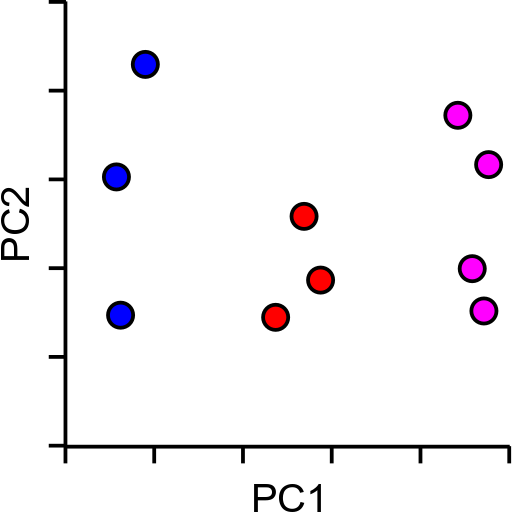
\includegraphics[width=1\textwidth,keepaspectratio]{images/dul/dim-reduce/pca-nonlinear-separation-1.png}
        \end{figure}
    \end{column}
    \begin{column}{0.5\textwidth}
        \begin{figure}
            \centering
            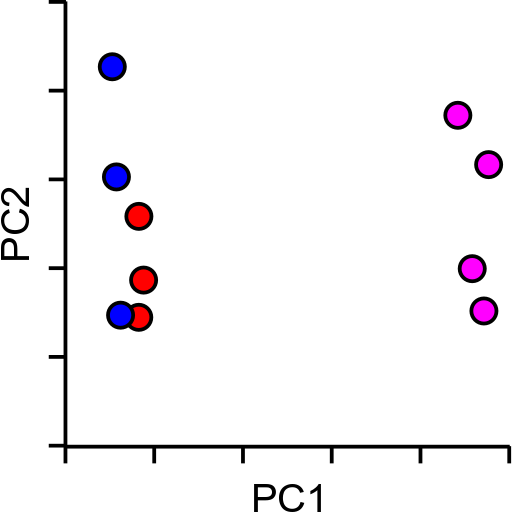
\includegraphics[width=1\textwidth,keepaspectratio]{images/dul/dim-reduce/pca-nonlinear-separation-2.png}
        \end{figure}
    \end{column}
    \end{columns}
    \begin{center}
        Non-linear separation of values
    \end{center}

    \framebreak

    Kind of\dots
    \begin{columns}
    \begin{column}{0.5\textwidth}
        \begin{figure}
            \centering
            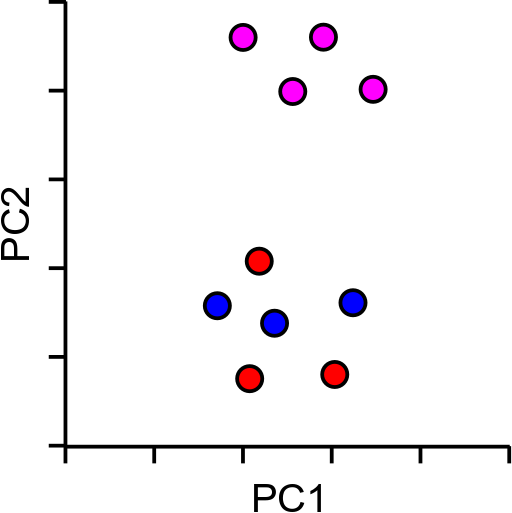
\includegraphics[width=1\textwidth,keepaspectratio]{images/dul/dim-reduce/pca-nonlinear-optimised-1.png}
        \end{figure}
    \end{column}
    \begin{column}{0.5\textwidth}
        \begin{figure}
            \centering
            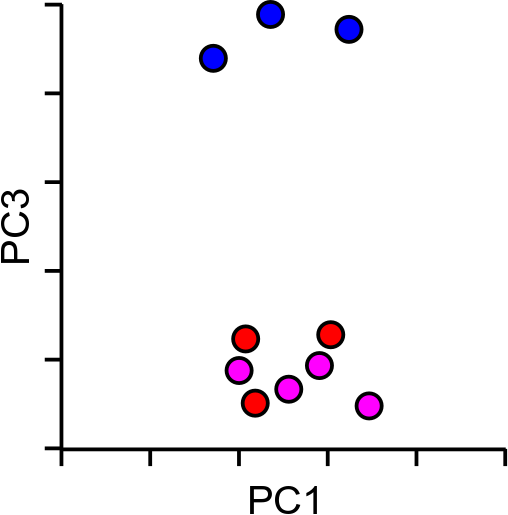
\includegraphics[width=1\textwidth,keepaspectratio]{images/dul/dim-reduce/pca-nonlinear-optimised-2.png}
        \end{figure}
    \end{column}
    \end{columns}
    \begin{center}
        Not optimised for 2-dimensions
    \end{center}
\end{frame}